\documentclass{SelimArticle}
%!TEX root = main.tex

%%%%%%%%%%%%%%%%%%%%%%%%%%%%%%%
% Additional Packages/Options %
%%%%%%%%%%%%%%%%%%%%%%%%%%%%%%%
% \setlist{nosep}
\hypersetup{hidelinks}

%%%%%%%%%%%%%%%%%
% Title Options %
%%%%%%%%%%%%%%%%%
\usepackage{mypage}
\school{McGill University}
\course{Computational Aerodynamics}
\coursenum{MECH 539}
%Add \\[0.3cm] for new line.
\title{Project 5}
\student{Selim \textsc{Belhaouane}}
\studentnum{260450544}
\date{\today}

%%%%%%%%%%%%%%%%%%%%%%%%%
% Additional Formatting %
%%%%%%%%%%%%%%%%%%%%%%%%%
%Horizontal line below section.
\sectionfont{\sectionrule{0pt}{0pt}{-5pt}{0.8pt}}
%Section numbering depth. Value of 2 means numbering ends with subsections.
\setcounter{secnumdepth}{3}
%Table of contents section depth. Same as above.
\setcounter{tocdepth}{2}
\numberwithin{equation}{section}
\numberwithin{figure}{section}

\newcommand{\ra}[1]{\renewcommand{\arraystretch}{#1}}
\begin{document}
\mytitlepage
\newpage
% Begin writing here.

\section{Solver Parameters}
The code for this project as well as the raw results were generated prior to the addendum, which
specifies values for freestream temperature $T_\infty$, freestream pressure $P_\infty$ as well as
the gas constat $R_{gas}$. It is important to note that all results below were generated
with the following parameters instead:
\begin{description}
    \item[$T_{0,\infty}$]: 1 (Stagnation Freestream Temperature)
    \item[$R_{gas}$]: 1
    \item[$P_\infty$]: 1
\end{description}

Moreover it is relevant to state that the code was written in Fortran 90 using double precision
and was compiled with a GNU Fortran compiler with the fastest optimization level (O3).

\section{Grids}
The coarsest grid was generated using the provided \texttt{generategrid.f90} with the following
parameters:
\begin{description}
    \item[\texttt{del\_min}]: 0.025
    \item[\texttt{imax}]: 80
    \item[\texttt{jmax}]: 40
\end{description}
Consequently, there are 40 evenly spaced grid points over the range of the airfoil.

The finer grids were generated by adding points at the midpoint of every existing grid point both
in the $x$ and $y$ direction. This resulted in a medium-sized grid and a finer grid, further
referred to as medium grid and fine grid respectively. For completeness, the number of grid
points for each grid is tabulated in~\Cref{tab:grids} below.

\begin{table}[H]
    \centering
    \caption{Grid specifications}\label{tab:grids}
    \begin{tabular}{@{} r c c @{}}
        \toprule
        Grid & Points in $x$ & Points in $y$ \\
        \midrule
        Coarse & 80 & 40\\
        Medium & 159 & 79\\
        Fine & 317 & 157\\
        \bottomrule
    \end{tabular}
\end{table}

\newpage
\section{Question 2}
\begin{quote}
    \textit{ Provide a plot of the pressure coefficient along the airfoil surface with the negative
    pointing upwards. Vary the freestream Mach number between [0.80, 0.90] with 0.02
increments. For each case, provide a convergence plot of the L$_\infty$-norm, surface pressure
coefficient as a function of $x$, and pressure contour for $x \in$ [20, 21] and $y \in $ [0, 1].
Discuss your findings. A four order reduction in the residual is sufficient for the Gauss-Seidel
method}
\end{quote}
Solver Parameters:
\begin{description}
    \item[Grid]: Fine
    \item[Solver]: Gauss-Siedel
    \item[Tolerance]: 1e-10
\end{description}

Surface pressure coefficient and convergence plots are provided in~\Cref{fig:q2_plots}.
Pressure contours are shown in~\Cref{fig:q2_contours}. It can be seen that increasing the
mach number has effects both on the convergence and on the location of the shock. These
are discussed in the following subsections.

\subsection{Shock location and intensity}
As shown in~\Cref{fig:q2_pressure}, increasing the inlet Mach number moves the shock
toward the trailing edge of the airfoil, as is expected: the flow needs to adjust
itself to match the back pressure.

Moreover, the shock intensity also increases with inlet Mach -- this can be seen from
the height of the pressure coefficient jump at the shock location. This phenomenon is also
expected: a larger Mach number right before a normal shock leads to a larger gain in
static pressure across the shock.

\subsection{Convergence}
\Cref{fig:q2_convergence} clearly shows the effects of Mach number on convergence: the higher
the inlet Mach number, the lower the convergence rate. In other words, more iterations
are required to converge as $M_{\infty}$ increases.

From a computational standpoint, there can be two explanations for this decrease
in convergence rate: the conditioning of the
matrix and the spurious variations in the matrix coefficients between iterations.

The conditioning of the matrix should not be expected to change significantly between
Mach numbers, as the coefficients still have relatively the same magnitudes. This is
confirmed by the fact that after around 20000 iterations all lines have approximately
the same slope, i.e. the same convergence rate. Thus, the main reason for the difference in
convergence time is due to the lower Mach number runs getting a "head start".

The lines for Mach numbers 0.88 and 0.90 show relatively large jumps in residual. These come from
the "sonic switches" turning off or on, which have a significant effect on the coefficient matrix,
and the difficulty in capturing the high intensity shocks.
coefficient matrix. The switches occur due to the hybrid nature of the Murman-Cole algorithm.

\begin{figure}
    \centering
    \begin{subfigure}{0.8\textwidth}
    \includegraphics[width=\textwidth]{./figs/q2_plots_1.pdf}
    \caption{Convergence.}\label{fig:q2_convergence}
    \end{subfigure}
    \\
    \begin{subfigure}{0.8\textwidth}
    \includegraphics[width=\textwidth]{./figs/q2_plots_2.pdf}
    \caption{Pressure distribution on airfoil surface.}\label{fig:q2_pressure}
    \end{subfigure}
    \caption{Effects of varying Mach number.}\label{fig:q2_plots}
\end{figure}

\begin{figure}[H]
    \centering
    \includegraphics[width=0.85\textwidth]{./figs/q2_contours}
    \caption{Contour plots for various Mach numbers.}\label{fig:q2_contours}
\end{figure}


\newpage
\section{Question 3}
\begin{quote}
    \textit{Vary the grid size, by doubling it in each direction as well as the number of points on
    the airfoil surface. Produce a coarse, medium, and fine grid. Plot the surface coefficient
of pressure as a function of x on the airfoil surface for the three grids on the same plot
at Mach 0.88. Discuss your findings. Does the shock location change.}
\end{quote}
Solver Parameters:
\begin{description}
    \item[Solver]: Gauss-Siedel
    \item[Tolerance]: 1e-10
\end{description}
The surface coefficient plots are shown in~\Cref{fig:q3}. It is expected that the shock would
approach a straight vertical line on the plot as the grid is refined merely due to plotting.
However, one may notice a shift in the shock location despite that fact; the center of the
shock moves slightly to the left as the grid is refined. This is especially noticeable
when comparing the coarse and medium grid results.

This error could be attributed to the truncation error of the scheme, which inevitably reduces
as the grid is refined.

\begin{figure}
    \centering
    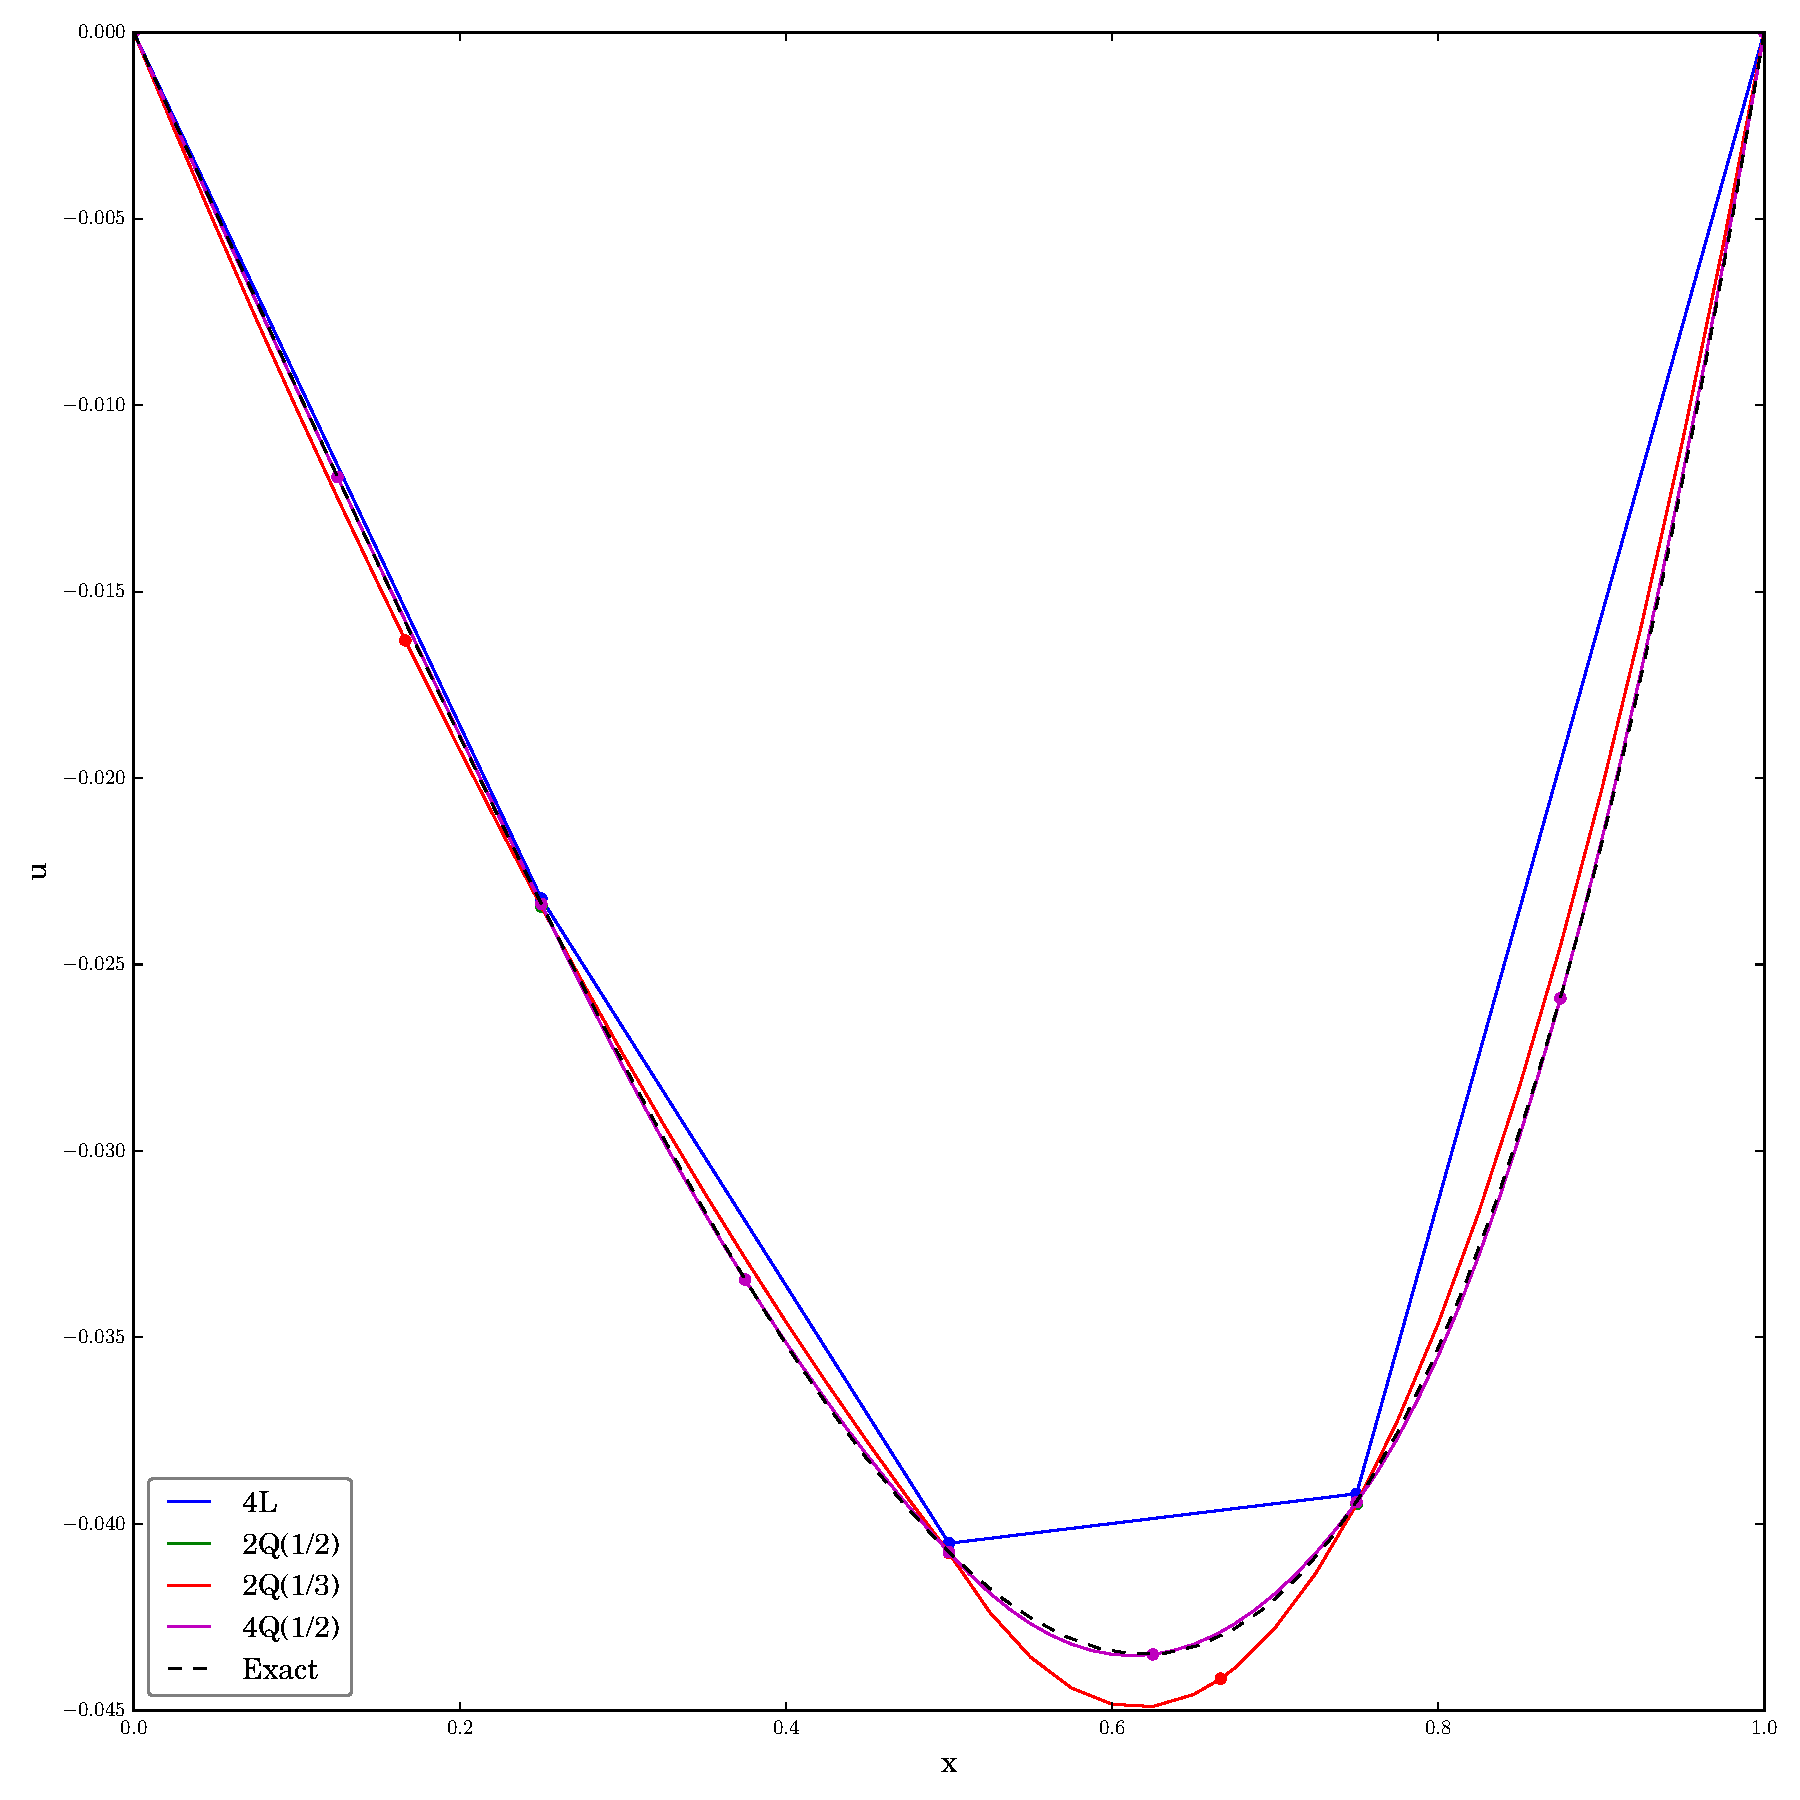
\includegraphics[width=0.8\textwidth]{./figs/q3}
    \caption{Pressure coefficient for various grids for $M_\infty$ = 0.88.}\label{fig:q3}
\end{figure}

\newpage
\section{Question 4}
\begin{quote}
    \textit{Now solve the equations using line implicit Gauss-Seidel at a Mach number of 0.86 and
    compare the convergence as a function of iterations and CPU time to that achieved by
the standard Gauss-Seidel approach. Both approaches must reach machine accuracy}
\end{quote}
Solver Parameters:
\begin{description}
    \item[Grid]: Coarse
    \item[Tolerance]: 1e-15
\end{description}
The convergence plots for Gauss-Siedel (GS) and Line-Implicit (LI) are shown in~\Cref{fig:q4}.
Moreover, quantitative results are summarized in~\Cref{tab:q4}.

\subsection{Convergence rate}
The steady convergence rate, the convergence rate after around 20000 iterations, is
higher for LI, as evidenced by the steeper slope. Moreover, jumps in residual are not
observed for the Line-Implicit scheme, further accelerating overall convergence.

\subsection{Time}
The Line-Implicit requires solving a tridiagonal system on each $j$ line. While this is
one of the cheapest linear systems to solve, it is still more expensive than the regular
Gauss-Siedel method. This explains the difference in \textit{time per iteration}.

However, in this case the price to pay is worth the reward: a lower time to convergence.

\subsection{Memory Footprint}
There is no substantial difference in memory footprint between the methods. Even though LI requires
storing vectors corresponding to the diagonal, lower and upper sub-diagonals as well as a right-hand
side vector, these are only of dimension \texttt{jmax}. In other words, an increase in memory
of approximately four vectors of length \texttt{jmax} is small compared to the cost of storing
$\phi$ as well as all the coefficients, which are all matrices of size \texttt{(imax,jmax)}.

\begin{table}[H]
    \centering
    \caption{Effect of solver on convergence. Values are normalized with respect to each metric
        in such a way that 1.0 is always the best value.}
    \label{tab:q4}
    \begin{tabular}{@{} r c c c @{}}
    \toprule
    Solver & Time & Iterations & Time per Iteration \\
    \midrule

GS & 1.35 & 1.70 & 1.00 \\
LI & 1.00 & 1.00 & 1.26 \\

    \bottomrule
\end{tabular}
\end{table}

\begin{figure}[H]
    \centering
    \includegraphics[width=\textwidth]{./figs/q4}
    \caption{Convergence of Line-Implicit and Gauss-Siedel solvers on the coarse grid.}\label{fig:q4}
\end{figure}

\section{Question 5}
Everything was answered in Question 2.

\end{document}
